% !TEX root = ../../../main.tex
% 来源：中学数学实验教材·第三册（高中数学）
% 章节：函数及其图象 / 一次函数（线性函数）
% 原始文件：4.tex，行 1556-1576
% 类型：tikz
% ---
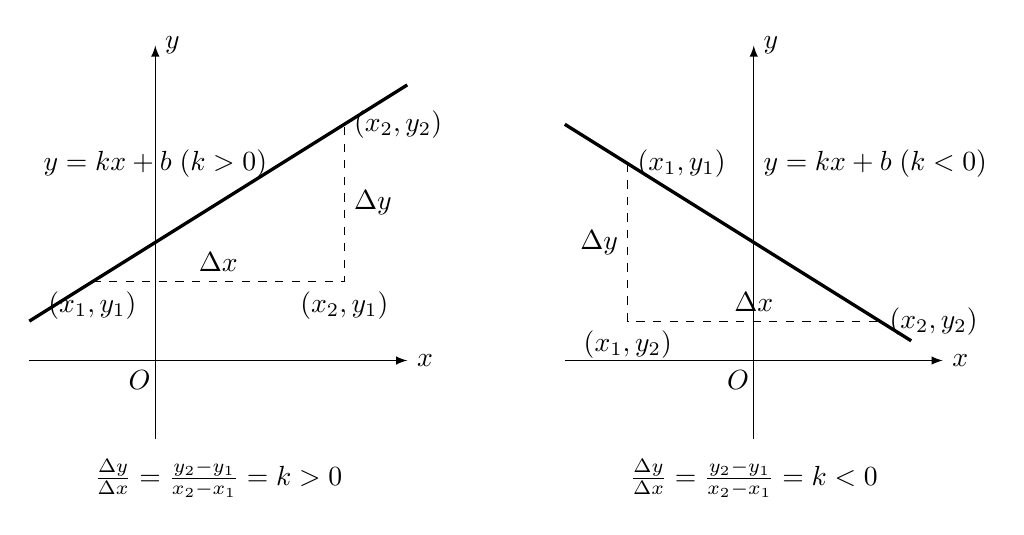
\begin{tikzpicture}[>=latex, xscale=.8, yscale=1]
\begin{scope}
    \draw[->](-2,0)--(4,0)node[right]{$x$};  
    \draw[->](0,-1)--(0,4)node[right]{$y$};
    \node at (-.25,-.25){$O$};
\draw [domain=-2:4, samples=10, very thick] plot(\x, {0.5*\x+1.5});
\draw[dashed](-1,1)node[below]{$(x_1,y_1)$}--node[above]{$\Delta x$}(3,1)node[below]{$(x_2,y_1)$}--node[right]{$\Delta y$}(3,3)node[right]{$(x_2,y_2)$};
\node at (0,2.5){$y=kx+b\; (k>0)$};
\node at (1,-1.5){$\frac{\Delta y}{\Delta x}=\frac{y_2-y_1}{x_2-x_1}=k>0$};

\end{scope}
\begin{scope}[xshift=9.5cm]
    \draw[->](-3,0)--(3,0)node[right]{$x$};  
    \draw[->](0,-1)--(0,4)node[right]{$y$};
    \node at (-.25,-.25){$O$};
    \draw [domain=-3:2.5, samples=10, very thick] plot(\x, {-0.5*\x+1.5});
    \draw[dashed](-2,2.5)node[right]{$(x_1,y_1)$}--node[left]{$\Delta y$}(-2,.5)node[below]{$(x_1,y_2)$}--node[above]{$\Delta x$}(2,.5)node[right]{$(x_2,y_2)$};
    \node at (0,2.5)[right]{$y=kx+b\; (k<0)$};
    \node at (0,-1.5){$\frac{\Delta y}{\Delta x}=\frac{y_2-y_1}{x_2-x_1}=k<0$};
\end{scope}
\end{tikzpicture}    
